\chapter{Introduction}
\label{ch1}

%%%%%%%%%%%%%%%%%%%%%%%%%%%%%%%%%%%%%%%
% IMPORTANT
\begin{spacing}{1.25} %THESE FOUR
\minitoc % LINES MUST APPEAR IN
\end{spacing} % EVERY
\onehalfspacing % CHAPTER
% COPY THEM IN ANY NEW CHAPTER
%%%%%%%%%%%%%%%%%%%%%%%%%%%%%%%%%%%%%%%

\section{Background}

Since the 18th century, iron, steel, and concrete have replaced timber and stone in the design, manufacture, and construction of large modern structures, including bridges. In the case of steel structures, components are factory-manufactured and then delivered to the construction site, where they are assembled or connected on site. Units are transported in members that are manufactured in factories. The members consist mostly of steel plates, and the main objective is to connect them together through a process called 'splicing'.

Steel bridges constructed between 1860 and 1955 were predominantly connected with riveted joints \cite{Quentin2012MorphogenesisStructures, COLLETTE2014, Ambroziak2023CASEANALYSIS, Collette2012Les18401940, Costa2013RehabilitationBridge}, as shown in Fig.\ref{fig-intro1} (Photo by Luca Upper \cite{lucaphoto}). In Japan, the period of cast iron started in 1897 which later shifted towards steel industry. The joints were riveted until the introduction of welding in the 1950s, where 40 kg grade SS39A and SS41 structural steel were used \cite{rivet1934}. This ancient type of joint allows secure connection of two or more metal sheets. Rivets are placed in the hole, then heated to high temperature by a pneumatic hammer which forms a head. After it cools down, a residual clamping force is created, making a riveted joint possible.

\begin{figure}[htbp]
    \centering
    
\includegraphics[width=0.85\textwidth]{imgs/intro/steel-structure.jpg}
    \caption{Riveted joint of railway bridge in Switzerland (Photo by Luca Upper)}
    \label{fig-intro1}
\end{figure}

After 1955, advancements in steel technology enabled the production of high-strength steel. As a result of the bolt's ease of construction and its reliable mechanical transmission mechanism, it quickly supplanted the rivet as the prevailing joining method.

\ac{HSB} have three types of connection: friction connection, bearing connection, and tension connection. Out of these, the friction connection is the most commonly used.

Friction connections involve joining materials that transmit stress through frictional resistance generated by the inter-material compressive force produced when the jointing materials are tightened using high-strength bolts. Stress is transferred via compressive forces between materials that are dispersed around the bolt, unlike in riveted joints where stress is transmitted through local bearing forces. This results in decreased stress concentration and smoother flow of stress. Another advantage is there is no misalignment between the joined materials until the application of a force which exceeds the frictional resistance can cause the friction to break and slip to occur, thus ensuring exceptionally high rigidity and fatigue strength.

Welding was first applied to steel bridges in the 1930s \cite{ALENCAR2019154}. And arc welding was first invented in the late 19th century, with high-density energies, like electron and laser beams, being applied to welding in the late 20th century. Welding conncetions are usually carried out in the factory due to the stringent construction conditions on site.

%todo!

%Insert 3 type of joint
Each of the three different types of connection has its own advantages and disadvantages, and no combination can completely replace any of them. And occasionally it is necessary to use two different types of joint at the same time, probably because of the lack of skilled labour (for repair riveted bridge, rivet combined with HSB), the inability of the joint surface to meet the required slip coefficients (Friction type combined with Bearing type connection) as well as the need to increase the strength of the joint to shorten the joint length (HSB combined with welded connection), etc.

%hybrid history


\begin{figure}
    \centering
    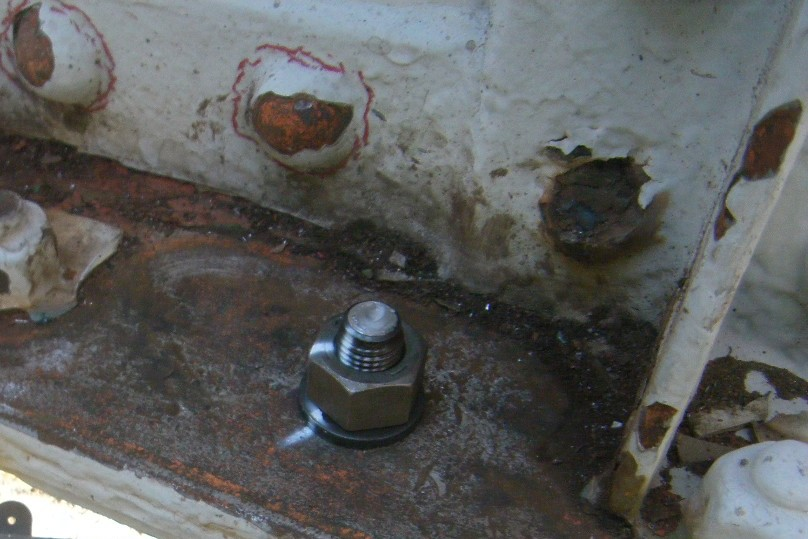
\includegraphics[width=0.8\textwidth]{imgs/intro/HSB-rivet.JPG}
    \caption{Rivet partially replaced by HSB of Hazukawa Riveted bridge in Fukui Japan}
    \label{fig-tprivet}
\end{figure}


\section{Technical Problem}

During the reconstruction projects following the Second World War, the combined use of diverse connection methods with varying principles presented challenges. For instance, when reinforcing aging riveted structures by welding or partially replacing them with \ac{HSB}, difficulties arose as shown in Fig. \ref{fig-tprivet}. Joining components with combined different load transfer mechanism connection methods results in a non-stationary structure, making it difficult to accurately calculate the sharing of loads in the past. As a result, only one of the two types was considered valid for design purposes at the time, ignoring the cooperative actions expected from their combined use.

The maintenance and repair of ageing bridges are expected to encounter growing obstacles in the near future. Bridges must achieve a compromise between suitable flexibility and rigidity. The addition of reinforcing elements to a completed bridge may upset this equilibrium and create problems. Consequently, post-construction reinforcement of a bridge may present a challenge by using hybrid connection.

In addition, for new structural components, the rational use of hybrid joints can effectively improve the strength of the joints and shorten the length of the joints as much as possible, while meeting the required strength to make the joint compact.  However, unlike the reinforcement of an existing structural component, new structural components raise issues of structural stability, durability and strict requirements for allowable deformation, and require a series of tests before they can be installed.

In summary, this work focuses on the following technical issues:

\begin{itemize}
    \item The primary technical challenge lies in the lack of understanding regarding the load transfer mechanism when combining connections with different mechanical principles.
    \item For the use of hybrid joints, not only to understand how the load is transmitted, but also to understand how the fasteners should be reasonably arranged. Different arrangements may produce different load transfer effects, so exploring the reasonable fastener arrangement scheme will be an important technical problem.
    \item The stiffness of Friction connection and bearing connection are different. In the case of a friction connection, there will be a small elastic dislocation (slip) before occurrence, which is a different mechanical mechanism from the elastic deformation of a bearing connection. Exploring the deformation capacity of the bearing and friction combination is also an important technical subject.
    \item After understanding the load transfer mechanism, strength and deformation performance of hybrid connections, it is necessary to define their limit states and to devise how to differentiate between the limit states and their corresponding strength equations.
    
\end{itemize}



\section{Aims and Scope}

This work is separated into two sections. The initial section entails repairing and enhancing aging riveted bridge through the replacement of damaged rivets with high-strength bolts using a friction connection. This technique is deployed to create hybrid joints that can jointly resist loads. The second section discusses the use of hybrid joints in the construction of new bridges. Such bridges encounter various design challenges, including the need to enhance component strength in response to increased external live loads without enlarging the structure size. These adjustments have become necessary in recent years, coinciding with the emergence and use of high-strength steels. The joints should be designed to withstand the increased strength of the steel components. However, the strength of friction joints is dependent on the number of bolts and slip coefficient. Enhancing the slip coefficient can effectively increase the joint strength, but this is an uncontrollable factor with significant construction costs. Therefore, it is imperative to suggest a cost-effective means of enhancing joint strength in high-strength steel structures without enlarging the joint size.
%本工作大体分为两个部分,第一个部分为(现存)老旧铆钉桥接头的补修补强,通过用高强螺栓替换部分已经损坏的铆钉以达到混合接头共同抵抗载荷的作用。第二部分为新建桥梁混合连接的应用,新建桥梁会面临很多设计合理性的问题,比如在外部活荷载日益增多的情况下如何在不增大桥梁结构的同时增强其部件的强度是近几年需要面临的调整,伴随着高强度钢的出现与应用,其接头也应当随着钢部件强度的上升而提高,然而摩擦接合的强度取决于螺栓的数量和滑移系数,滑移系数的提高能有效增强接头的强度,然而滑移系数是不可控且施工成本很高。因此需要提出一种低廉的可以增强接头强度的接合方法来应对高强度钢结构。

Investigating the riveted joint contact surfaces of aging riveted bridges is necessary to provide a reliable slip coefficient for the friction connection, which is essential in calculating the strength of hybrid joints consisting of rivets and high-strength bolts in existing steel structures. This is because high-strength bolt friction connections resist loads through friction at the interface. When replacing the rivets, it is important to take special care during removal as the rivets may still be sharing part of the load, particularly in areas where there is more load sharing. It must be ensured that the load originally resisted by the rivets is appropriately transferred to other rivets to avoid potential damage to neighbouring rivets. Hence, an examination of the method by which the load is distributed within riveted joints, both with and without a specific damaged rivet, and replacing it with high-strength bolts is essential. The removal of a rivet affects the mechanism of load redistribution, necessitating careful consideration in the bolt arrangement to ensure that high-strength bolts can aptly withstand external forces.  Once the principle of redistributing the load after removing individual rivets is understood, it becomes necessary to systematically arrange high-strength bolts and explore the load transfer mechanism of the hybrid joint. The high-strength bolts exhibit high stiffness and distinct deformation performance from riveted joints, necessitating an investigation into the deformation performance of the Rivet-HSB hybrid connection. Also, it is essential to investigate the load-carrying capacity of hybrid connections and establish a limit state in accordance with the allowable deformation value.

For hybrid connections composed of a combination of rivets and high-strength bolts, this study concentrates on achieving the following aims:

\begin{enumerate}
    \item Provide reliable slip coefficients for riveted connections
    \item Investigate the mechanism of load redistribution after removing individual rivets
    \item Investigate the load transfer mechanism and deformation performance of hybrid rivet-\ac{HSB} connections
    \item Differentiation of limit states and proposal of strength calculation formulas
\end{enumerate}
%首先是对于现存钢结构的铆钉和高强螺栓的混合接头,由于高强螺栓摩擦接头是通过界面的摩擦来抵抗载荷的,因此调查老旧铆钉桥的接合面是有必要的,需要为摩擦结合提供一个可靠的滑移系数以计算接头的强度。然后再更换铆钉时,由于铆钉可能仍然分担着一部分力,特别是对于载荷分担比较多的区域,在拆除铆钉时需要特别注意原本铆钉抵抗的这部分力会转移到其他铆钉上,这有可能会造成相邻铆钉发生损坏,因此,在用高强螺栓部分更换铆钉时有必要调查清楚铆钉接头的载荷分担方式以及拆除某一个铆钉时,载荷会如何进行再分配,从而可以更好的进行配置高强螺栓,使得高强螺栓能合理的承载尽可能多的外力。了解了拆除个别铆钉后才分配原理之后,就需要合理的进行安排高强螺栓,并探讨结合了高强螺栓的混合接头的力学传递机理以及其变形能力,由于组合了刚度较高的高强螺栓,因此其变形能力和铆钉接头会有所区别,探讨其承载能力以及根据形变量来定义一个极限状态是必须的。
%对于铆钉和高强螺栓组合成的混合接头,本工作着重解决以下几个目标:
%1. 铆钉接合面的滑移系数
%2. 拆除铆钉时,铆接的再分配原理
%3. 铆钉-高强螺栓混合接头的力学传递机理及其变形能力
%4. 极限状态的区分以及强度计算式的提案

Secondly, for newly constructed steel bridges, bearing-type connections as substitutes for rivets have emerged as interference-fit bolts. In recent years, research on injection bolts and high-strength mechanical rivets has also progressed. This work focuses on the discussion of interference-fit bolts as bearing-type connections and a combination of high-strength bolt friction connections. The development and proposal of such hybrid connections were the main research objectives of this work. The feasibility of the hybrid connection will be explored first through numerical analysis, where, although the mechanical transmission mechanism is unknown, the approximate joint strength can still be obtained through simple accumulation of each fastener (unlike the hybrid connection of welding and high-strength bolts, the connection strength cannot be calculated by accumulation, which will be explained in detail in Section \ref{sec-hsbweld}). Secondly, if pretension is applied to the interference fit bolts,the bolts are tightened, and the tensioned part of the shaft may produce small gaps with the bolt hole wall. The mechanism by which pretension affects the bearing resistance of the interference fit bolts needs to be explored. Similar to the hybrid connection between rivets and high-strength bolts, the deformation capability of IFB and HSB hybrid joints also needs to be discussed. Owing to the higher pretension applied to the IFB and its different material properties compared to rivets, the deformation performance may vary. The purpose of this work is to explore the deformation performance of the connection, define its ultimate state, and propose a strength calculation equation based on theoretical, experimental, and analytical results.

%其次是对于新建钢结构来说,承压型接作为铆钉的替代过盈配合螺栓最早出现,近几年注射螺栓以及机械式高强铆钉的研究也出现了进展,本工作着重探讨过盈配合螺栓作为承压型连接和高强螺栓摩擦连接组合成混合连接,发展并提案此类混合连接是本工作的重点研究,研究首先会通过数值解析探讨混合连接的可行性,尽管不知道力学传递机理,但是依然可以通过简单的承载力累加得出大概的接头强度(这与焊接和高强螺栓的混合连接不同,后者无法通过累加的方式来计算获得接头的强度,在之后的章节\ref{sec-hsbweld}会进行详细的解释)。其次如果对过盈配合螺栓如果施加预紧力,螺栓则会产生紧缩效应,轴部紧缩后的螺栓可能会与螺栓孔壁产生微小的缝隙,预紧力是否会影响过瘾配合螺栓承压抵抗的机理有待探讨。和铆钉-高强螺栓混合接头一样,IFB和HSB的混合接头一样需要讨论其接头的形变能力,由于IFB会施加较高的预紧力,且其材料特性和铆钉不太一样,因此形变能力也会有所差别,探讨接头的变形能力,定义其极限状态,并通过理论,实验,解析结果分析并提案一个强度计算式是本工作的目的。

%对于IFB和HSB组合的混合接头,本工作着重解决以下几个目标:
%1. 混合接头的可行性研究
%2. IFB施加预紧力给承压连接带来的影响
%3. 探讨IFB-HSB混合接头的力学传递机理,及其形变能力,并给出最合适的螺栓配置方案。
%4. 极限状态的区分以及强度计算式的提案

%最后需要总结两种不同的承压连接和摩擦连接的混合接头,并总结分析提出一个混合接头的极限状态设计法是本工作的最终目标。

For the hybrid connection of IFB and HSB, this work focuses on the following objectives: 

\begin{enumerate}
    \item Feasibility study of the hybrid connection. 
    \item Investigation of the effects of preload for IFB on bearing-type connections.
    \item Exploration of the load transmission mechanism and deformation performance of the IFB-HSB hybrid connection, and provision of the most suitable bolt arrangement plan.
    \item Differentiation of the limit state and proposal of a strength calculation formula.
\end{enumerate}

Lastly, it is necessary to summarize and analyze the hybrid connections of the two different bearing-type connections and friction-type connections, and to propose a design method for the limit state of the hybrid connection and the strength calculation formula. This is the ultimate goal of this work.





\section{Research Approach And Thesis Outline}

Firstly, the theoretical background on bearing-type and friction-type connections will be reviewed, followed by an exploration of installation methods and material properties of fasteners.

Based on this literature review, a preliminary selection will be made on the important parameters in the choice of alternative products to be further investigated, such as the type of fastener. Then, taking the information from literature as a basis, the conditions required for hybrid joints are explored in detail and a computational model is proposed to evaluate the method for strength calculation as well as the mechanical distribution mechanism of hybrid joints.

The main body of this research project is based on the fundamental approach of numerical analysis and experiment. Conduct a finite element analysis project to investigate the load transmission mechanism using Abaqus analysis software. Test hybrid joints with partially replaced HSB under riveted joints and hybrid joints with high strength bolts combined with IF bolts to validate the analysis results. This will be performed by testing double lap shear connections with Rivet \& \ac{HSB} or \ac{IFB} \& HSB in the Osaka Metropolitan University Mechanical Laboratory.

Finally, the results obtained from the double lap shear tests and analysis are processed to gain the load transfer mechanism, hybrid joint strength and the condition of limit state.

Lastly, the test results obtained will be used to propose a limit state design method for the hybrid joint combined bearing and friction type connection.

The study's purpose was broadly categorised into three objectives: 1) Clarify the Mechanics Behaviour of Bearing and Friction Hybrid Joint, 2) Define the limit state for the hybrid joint, and 3) Propose design methods and strength equations. An overview of the steps taken in this research project is shown in the diagram on the following page as shown Fig. \ref{fig-rflow}.

%research flow
\begin{figure}
    \centering
    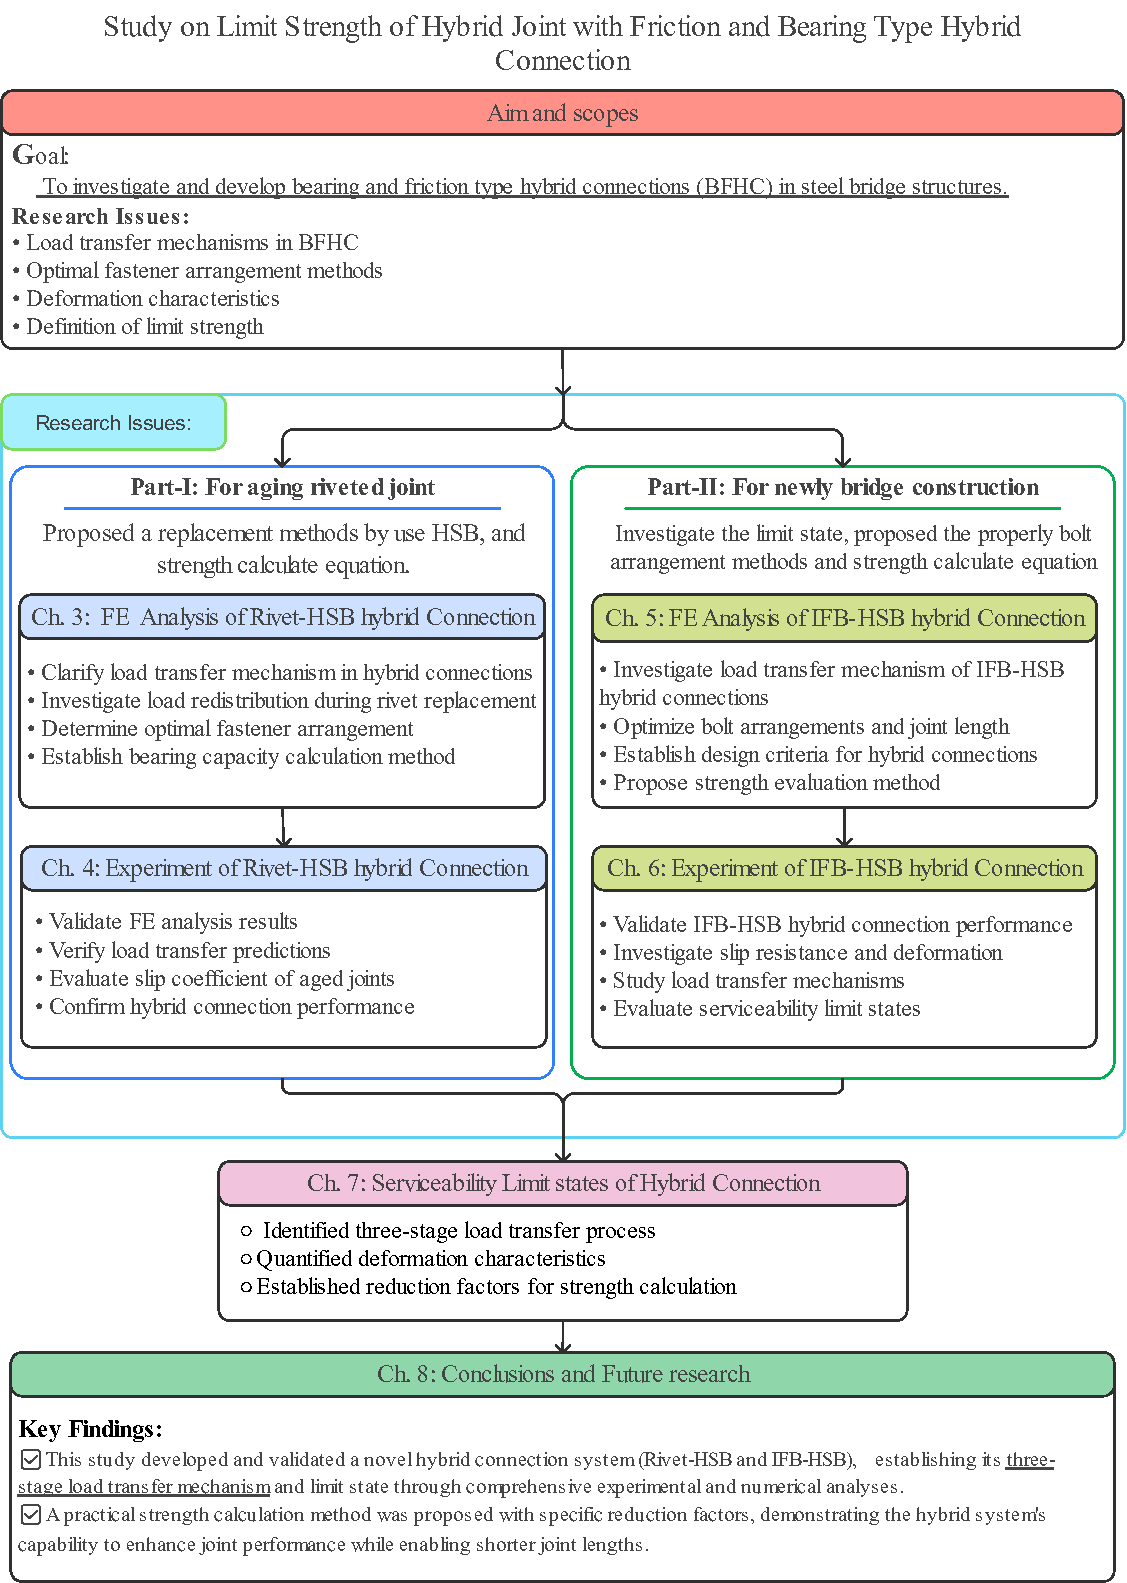
\includegraphics[width=\textwidth]{imgs/intro/research-flow.pdf}
    \caption{Overview of work flow of this research project}
    \label{fig-rflow}
\end{figure}